\ifdefined\included
\else
\setcounter{chapter}{2} %% Numéro du chapitre précédent ;)
\dominitoc
\faketableofcontents
\fi

\chapter{Models and Algorithms for human-aware task planning with integrated theory of mind}
\chaptermark{Models and Algorithms of Theory of Mind}
\label{chap:3}
\minitoc


%%% SECTION %%%%%%%%%%%%%%%%%%%%%%%%%%%%%%%%%%%%%%%%%%%%%%%%%%%%
\section{Introduction}



\begin{figure}
    \centering
    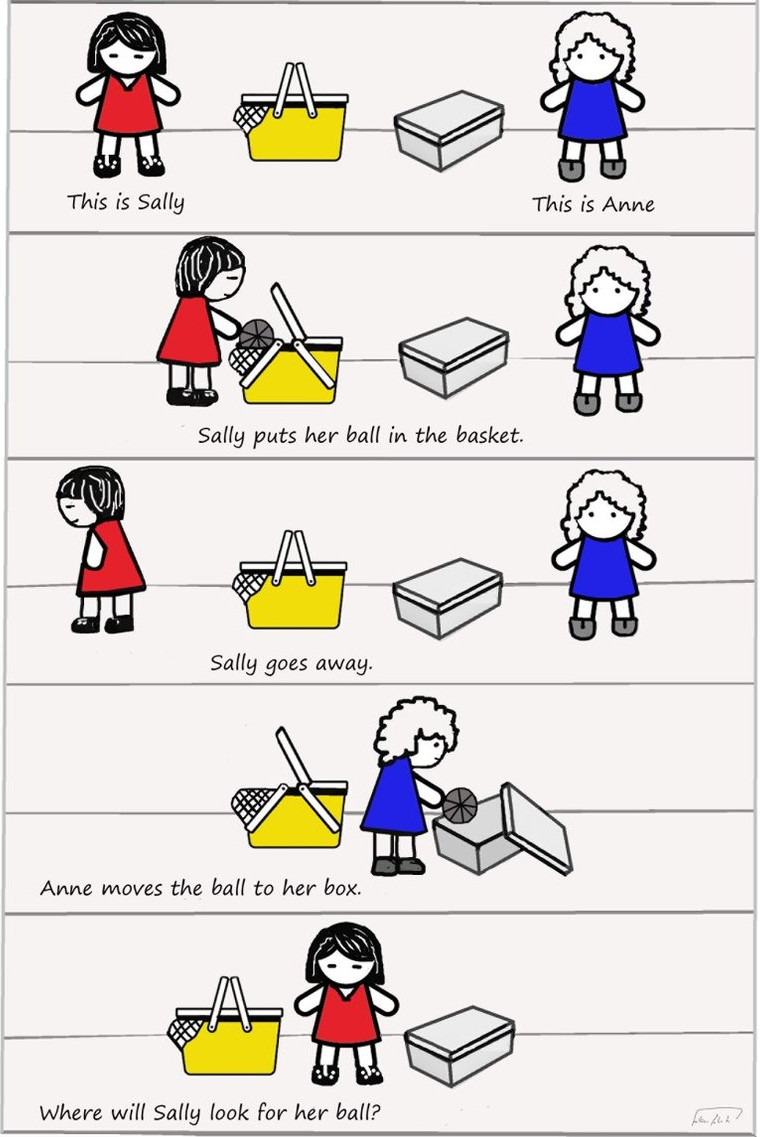
\includegraphics[width=0.5\linewidth]{images/Chapter3/The-Sally-Anne-Task.jpeg}
    \caption{Sally and Anne Task}
    \label{fig:sally_and_anne_task}
\end{figure}

False beliefs tasks are commonly used tests to acknowledge the presence of Theory of Mind reasoning. The most common test is the \textit{Sally and Anne} one, depicted in fig~\ref{fig:sally_and_anne_task}, and is used in developmental psychology to examine children's "theory of mind" understanding, which refers to their ability to understand how other people think, feel and behave. The test consist in describing the execution of a simple task involving non-observable objects and co-presence, then children are questioned about the belief of one of the character. The task consist in the following. Sally and Anne are two co-present characters near a basket and a box. Sally puts her ball in the basket before going away. Then, Anne moves the ball from the basket to the box, in hindsight of Sally. Eventually, the question is where will Sally look for the ball she left? As an observer of this scene, using Theory of Mind, we can naturally say that Sally will look for her ball in basket because she isn't aware that Anne moved the ball in the box. Very young children are not able to understand that Sally isn't aware of Anne's action and thus, they are likely to answer that Sally will look in the box. 

Theory of Mind reasoning is a very important skill for \textit{good} interaction and collaboration between agents. Thus, it is reasonable and desirable to aim at endowing robots with such skill to enhance their interactions with humans. This is the motivation of the contribution presented in this chapter. Here, we propose an extension of HATP/EHDA to be able to maintain in a principled way the human beliefs during the planning process, and to tackle estimated false human beliefs that may be detrimental to the task resolution.

We would want the robot to be able to reason and maintain correctly the distinct human beliefs. Despite modeling distinct beliefs, HATP/EHDA doesn't maintain in a principled way, only in a scripted way (domain specific). Here we propose some models and algorithms to integrate some concept of Theory of Mind in the planning process of HATP/EHDA. This way, the robot can estimate more accurately the human's belief to predict their behavior. Moreover, we propose solutions for the robot when to tackle estimated false human beliefs that may impact the task resolution.




%%% SECTION %%%%%%%%%%%%%%%%%%%%%%%%%%%%%%%%%%%%%%%%%%%%%%%%%%%%
\section{Related works}

    This chapter's contribution is related to several topics not mentioned yet. Hence, to better capture the contribution, this section introduces the new topics and relevant related works.  

    %%% SUB-SECTION %%%%%%%%%%%%%%%%%%%%%%%%%%%%%%%%%%%%%%%%%%%%
    \subsection{Epistemic planning}
    Epistemic planning plays a crucial role in human-robot collaboration. It allows robots to reason about their own knowledge and beliefs, as well as the knowledge and beliefs of other agents \cite{bramblett_epistemic_2023}. This is important for coordination and collaboration among multiple agents, as success can only be expected if agents can reason about each other's knowledge, uncertainty, and capabilities \cite{bramblett_epistemic_prediction_2023}. Epistemic planning is used in various application areas, including mobile service robots, explaining planning, game playing, human-robot interaction, and social robotics \cite{hu_planning_2023}. It enables robots to make plans to achieve the required knowledge and to reason about the knowledge and capabilities of other agents, ensuring effective collaboration and coordination in human-robot interactions \cite{belle_epistemic_2023}.


    Def. Thomas Bolander is one of the main contributor to this field. Proposed the DEL approach. \cite{bolander_gentle_2017} and extended it.

    ``Automated planning is a branch of artificial intelligence concerned with computing plans (sequences of actions) leading to some desired goal. A human or robot could e.g. have the goal of picking up a parcel at the post office, and then the problem becomes to find a successful sequence of actions achieving this. Epistemic planning is the enrichment of planning with epistemic notions, that is, knowledge and beliefs. The human or robot might have to reason about epistemic aspects such as: Do I know at which post office the parcel is? If not, who would be relevant to ask? Maybe the parcel is a birthday present for my daughter, and I want to ensure that she doesn't get to know, and have to plan my actions accordingly (make sure she doesn't see me with the parcel). The epistemic notions are usually formalized using an epistemic logic. Epistemic planning can naturally be seen as the combination of automated planning with epistemic logic, relying on ideas, concepts and solutions from both areas.''

    Muise et al. worked on multi-agent epistemic planning using a classical planning approach. Since involving nested beliefs is computationally demanding, their work proposes to convert and encode such problems into classical planning problems. Hence, state-of-the-art classical planning technics can be used to tackle nested beliefs of multiple agents problems. 

    \subsection{Theory of Mind in HRC}
    Epistemic planning helps to plan the correct sequence of actions to perform to reach a desired knowledge, including a desired world state. However, estimating the current knowledge and beliefs of the different agents is challenging. To do so, we have to consider Theory of Mind concepts, especially perspective shift and the notion of co-presence. Some epistemic planning works already integrate of ToM notions, but the subject is worth being discussed a bit more in details. Indeed, in the HRI field, ToM is used in various domains like navigation, dialogue and like here in task planning. 

    Theory of mind (ToM) plays a crucial role in task planning for human-robot collaboration. 
    ToM refers to the ability to attribute mental states to oneself and others, such as beliefs, desires, and intentions. 
    
    (v1) Robots endowed with ToM abilities can anticipate and understand the mental states of their human partners, allowing for more effective interaction and decision-making. By inferring their partner's trust and strategy, robots can adjust their own decision models and policies to optimize team performance [1]. Mimicking ToM in robots influences human decision-making behavior and trust, making it more appropriate and conducive to collaboration [2]. Robots implementing ToM are perceived as more socially intelligent and helpful, enhancing the quality of human-robot interactions [3]. Computational theory of mind, based on abstractions of beliefs into higher-level concepts, enables agents to reason and collaborate with humans efficiently, improving decision-making outcomes [4]. However, the field lacks a unified construct and consistent benchmarking, hindering progress in endowing robots with ToM capabilities [5].

    (v2) Robots endowed with ToM abilities are more effective in proactive robotic assistance and are perceived as more socially intelligent by humans \cite{shvo_proactive_2022}. ToM enables robots to infer human desires, beliefs, and intentions, allowing for natural interaction between robots and humans \cite{yu_robot_2023}. Robots with ToM can anticipate human strategies and incorporate them into their decision models, leading to better team performance \cite{romeo_exploring_2022}. The presence of ToM in robots influences human decision-making behavior and trust, making it more appropriate for human-robot collaboration \cite{schlobach_abstracting_2022}. Computational theory of mind, based on abstractions of beliefs into higher-level concepts, facilitates collaboration on decisions and improves the quality of human decisions \cite{gurney_robots_2022}. However, the lack of a unified construct and consistent benchmarking hinders progress in endowing robots with ToM capabilities.

    \textbf{TODO: Merge two versions, but references of v1 are not accessible anymore...}

    
    \subsection{Communication in HRC}

    Communication plays a crucial role in human-robot collaboration. It enables effective interaction between humans and robots, promoting inclusivity and reducing obstacles in human-robot interaction. Communication allows robots to share information about their actions and intentions, enhancing transparency and explainability \cite{mcmillan_human-robot_2023}. It helps in establishing trust and understanding between humans and robots, leading to improved teamwork and performance \cite{verhagen_influence_2022}. Non-verbal gestures and behavior of robots during collaboration can impact the perception of the robot and influence the willingness of humans to cooperate \cite{arntz_collaborating_2022}. Communication also allows robots to assess their own skills and limitations, propose alternatives, and adapt the execution of tasks to the capabilities of the collaborators \cite{ferrari_bidirectional_2022}. Overall, effective communication facilitates mutual knowledge, enables the exchange of information, and allows humans and robots to work together efficiently and successfully.


%%% SECTION %%%%%%%%%%%%%%%%%%%%%%%%%%%%%%%%%%%%%%%%%%%%%%%%%%%%
\section{Maintaining the human beliefs}

    %%% SUB-SECTION %%%%%%%%%%%%%%%%%%%%%%%%%%%%%%%%%%%%%%%%%%%%
    \subsection{Enhanced problem specification}

\textbf{TODO: switch from 'we' to 'I'?}

\begin{figure}[t!]
    \centering
    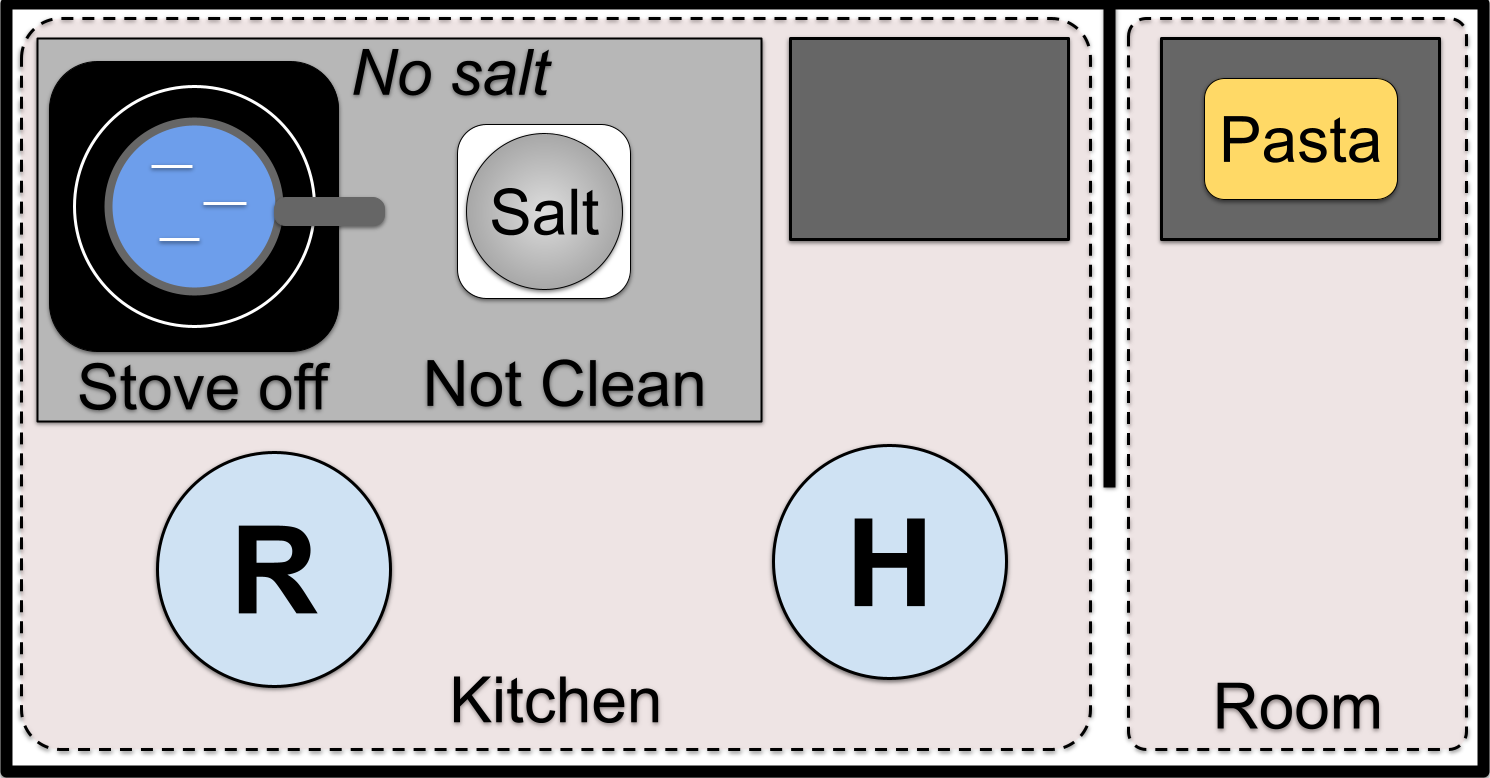
\includegraphics[width=0.70\linewidth]{images/Chapter3/cooking_task_draw.png}
    \caption{
    Let us consider cooking pasta as a human-robot shared task. 
    The robot has to turn on the stove (\textit{stoveOn}) and clean the counter (\textit{counterClean}), but the latter is not a part of the shared task. The human takes care of fetching the pasta while both agents can add salt into the water (\textit{saltIn}). Before pouring the pasta into the pot the human must know the facts, \textit{stoveOn} and \textit{saltIn}. 
    Unlike \textit{stoveOn}, the facts \textit{saltIn} and \textit{counterClean} are not directly observable. 
    Hence, by acting while the human is away to fetch the pasta, the robot may induce false beliefs which may be detrimental to the shared task (e.g., human adding salt again).
    }
    \label{fig:new_scene}
\end{figure}

We start from the HATP/EHDA probleme specification which is the following.

We consider a \textit{classical planning domain} (\textit{state-transition system}) $\Sigma = (S,A,\gamma)$, s.t., $S$ is a finite set of states in which the system may be, $A$ is a finite set of actions that the actors may perform, $\gamma : S \times A \rightarrow S$ is a state-transition function. Each state $s \in S$ is a description of the properties of various objects in the planner's environment~\cite{naubooks0014222}. 

To represent the objects and their properties, we will use two sets $B$ and $X$: $B$ is a set of names for all the objects, plus any mathematical constants representing properties of those objects. $X$ is a set of syntactic terms called state variables, s.t. the value of each $x \in X$ depends solely on the state $s$.

A \textit{state-variable} over $B$ is a syntactic term $x = sv(b_1, ..., b_k)$, where $sv$ is a symbol called the state variable's name, and each $b_i$ is a member of $B$ and a parameter of $x$. Each state variable $x$ has a range, $\textit{Range}(x) \subseteq B$, which is the set of all possible values for $x$.

Here is the description of the sets $B$ and $X$ for the collaborative cooking example:
{\small
\begin{align*}
&B           = Entities \cup Places \cup Booleans \cup \{\textsf{nil}\} \\
&\quad Entities    = Agents \cup Objects\\
&\quad Agents      = \{ \textsf{R}, \textsf{H} \} ~~ \backslash\backslash~\textsf{R}:robot,~\textsf{H}:human\\
&\quad Objects     = \{ \textsf{salt}, \textsf{pasta}, \textsf{counter} \}\\
&\quad Places      = \{ \textsf{kitchen}, \textsf{room} \}\\
&\quad Booleans    = \{ \textsf{true},\textsf{false} \}\\
&\\
&X = \{ at(e), saltIn, stoveOn, counterClean ~ | ~ e \in Entities \}\\
&\quad \textit{Range}(saltIn ~|~ stoveOn ~|~ counterClean)=Booleans\\
&\quad \textit{Range}(at(\textsf{R} ~|~ \textsf{H} ~|~ \textsf{pasta})) = Places\\
&\quad \textit{Range}(at(\textsf{salt} ~|~ \textsf{counter})) = \{ \textsf{kitchen} \}
\end{align*}
}

A \textit{variable value assignment} function over $X$ is a function $val$ that maps each $x_i \in X$ into a value $z_i \in$ $\textit{Range}(x_i)$. With $X = \{ x_1, ..., x_n \}$, we will often write this function as a set of assertions: $val = \{ x_1=z_1, \ldots, x_n=z_n \}$. 

Our first contribution starts from here where we augmented the specification by associating each state variable to a location and to an observability type.

A \textit{variable observability assignment} function over $X$ is a function $obs$ that maps each $x_i \in X$ into an observability type $t_i \in \{ \texttt{OBS},  \texttt{INF} \}$: $obs = \{ (x_1,t_1), \ldots , (x_n,t_n) \}$. Respectively, when $obs(x_i) = \texttt{OBS} | \texttt{INF}$ then $x_i$ is said to be \textit{observable} $|$ \textit{inferable} in the state $s_i$.

A \textit{variable location assignment} function over $X$ is a function $loc$ that maps each $x_i \in X$ into a $l_i \in Places \cup \{ \texttt{nil} \}$: $loc = \{ (x_1,l_1), ..., (x_n,l_n) \}$. 
$Places \subseteq B$ captures a group of constant symbols such that each member is a predefined area in the environment. 
Agents are always either ``situated'' in a place or moving between two places. 
We consider $x_i$ to be located in every $place \in Places$ if $loc(x_i)=\texttt{nil}$. 
More details about how the environment should be divided into places will be given shortly.

A \textit{state} $s_i \in S$ is a 6-tuple composed of 4 functions over $X$ and 2 task networks (agendas)  s.t. $s_i = (val_i, val^H_i, obs_i, loc_i, tn^R_i, tn^H_i)$. 
The state of the world from the perspective of the robot is captured by the variable value assignment function $val_i$, sometimes noted as $val^R_i$. 
Similarly, $val^H_i$ represents the estimation of $val_i$ in the perspective of the human, also referred to as the estimated human beliefs. 
Hence, $\forall s_i \in S$, each $x_j \in X$ is  mapped to two \textit{values} (robot perspective and estimation of human's beliefs), an \textit{observability type}, and a \textit{place}. We say that a state $s_i \in S$ contains \textit{false beliefs}, or \textit{belief divergences}, if $\exists x_j \in X, val^H_i(x_j) \neq val^R_i(x_j)$. 

For our example, the initial state $s_0$ would be as follow: 

{\small
\noindent
\begin{multline*}
s_0 = \{val_0, ~val^H_0, ~obs_0, ~loc_0, ~tn^R_0, ~tn^H_0\} \\ \quad
\end{multline*}
\bigvspace
\begin{multline*}
\quad val_0 = val^H_0 = \{at(\textsf{R}) = \textsf{kitchen}, at(\textsf{H}) = \textsf{kitchen},\\ 
at(\textsf{pasta}) = \textsf{room}, saltIn = \textsf{false}, stoveOn=\textsf{false} \}
\end{multline*}
\smallvspace
\begin{multline*}
\quad obs_0=\{ (at(e),\texttt{OBS}),
(saltIn,\texttt{INF}),
(stoveOn,\texttt{OBS})\\
(counterClean,\texttt{INF}),
~|~ e \in Entities \}
\end{multline*}
\smallvspace
\begin{multline*}
\quad loc_0=\{ (at(e),val_0(e)),
(counterClean,\textsf{kitchen}),\\
(saltIn,\textsf{kitchen}),
(stoveOn,\textsf{kitchen}),
~|~ e \in Entities \}
\end{multline*}
\smallvspace
\begin{multline*}
\quad tn^R_0 = \{ CookPasta, CleanCounter \} \\ \quad
\end{multline*}
\bigvspace
\begin{multline*}
\quad tn^H_0 = \{ CookPasta \} \\ \quad
\end{multline*}
\smallvspace
}

An action is a tuple $\alpha = (\textit{head}(\alpha), \textit{pre}(\alpha), \textit{eff}(\alpha))$ where $\textit{head}(\alpha)$ is a syntactic expression of the form $\textit{act}(z_1, ..., z_k)$ where $act$ is a symbol called the \textit{action name} and $z_1,...,z_k$ are variables called parameters. $\textit{pre}(\alpha) = \{ p_1, ..., p_m \}$ is a set of preconditions, each of which is a literal. And $\textit{eff}(\alpha) = \{ e_1, ..., e_n \}$ is a set of effects, each of which is an expression of the form: $sv(t_1, ..., t_j) \leftarrow t_0$ with $t_0$ being either the value to assign to the state variable $sv(t_1, ..., t_j)$ or a new location/place for the state variable. We note $\textit{agt}(\alpha)$ the agent performing the action $\alpha$.

To estimate the next possible actions that an agent $\varphi \in Agents$ is likely to perform in a state $s_i \in S$, we proceed in the same way as in~\cite{buisan:hal-03684211}. We refine the agent's agenda $tn_{\varphi}$ based on its belief $val^\varphi_i$ and obtain a \textit{refinement} as follows $\textit{ref}(tn^\varphi_i, val^\varphi_i)= \{ (a_1,tn_1),...,(a_j,tn_j) \}$. 
A \textit{refinement} contains a tuple for each estimated possible action $a_j$ and the associated new agenda $tn_j$ after being refined. 

In our cooking example, we obtain the following refinement if the starting agent is the human:\\
{\small
$\textit{ref}(tn^H_0, val^H_0) = \{ (add\_salt(),tn_1), (move\_to(\textsf{kitchen}),tn_2) \}$
}


    %%% SUB-SECTION %%%%%%%%%%%%%%%%%%%%%%%%%%%%%%%%%%%%%%%%%%%%
    \subsection{State Transitions and Beliefs Updates}
Learn from observation of either: action execution or observable state.

Assumption 1 : We do not consider uncertainties. Thus, agents are either wrong or right about the state of the world but never uncertain. This would be an interesting future work. 

Assumption 2 : We do not consider cases where the robot's beliefs can diverge. Since the planner is part of the robot, the actual ground truth is unknown. We can only assume that the estimation of the state of the world by the robot is correct and reason on it.

Assumption 3 : Coming from the two previous assumptions, we assume that the human only makes deterministic moves when not being observed. Hence, regardless of being co-present, the robot's beliefs are always updated with the action's effects.


Thus, $\forall x \in X$, we always have,

\begin{equation}
    val_{i+1}(x) = \left\{ 
    \begin{array}{ll}
        w, & \mbox{if} ~ x \leftarrow w \in \textit{eff}(a)   \\ 
        val_i(x), & \mbox{otherwise}
    \end{array}\right.
\end{equation}

The place associated with a state variable can be modified by the action's effect but, here, we assume that the observability type of each fact is constant during the task. So, $\forall x \in X$,

\begin{align}
    &obs_{i+1}(x) = obs_i(x)\\
    &loc_{i+1}(x) = \left\{ 
    \begin{array}{ll}
        l, & \mbox{if} ~ x \leftarrow l \in \textit{eff}(a)\\
        loc_i(x), & \mbox{otherwise}
    \end{array}\right.
\end{align}

The new agenda of each agent ($tn^R_{i+1}, tn^H_{i+1}$) are created by the HTN refinement algorithm, and thus, they are directly retrieved from the obtained refinement. 
This refinement decomposes abstract tasks in the task network until the first task is a primitive action. To do so, every applicable method is applied leading to a set of possible actions (and refined task networks).

The new estimated human belief $val^H_{i+1}$ is the two-step result of our Situation Assessment processes that models the human's real-time sensing and reasoning capabilities about their surroundings.

First, let us define the notions of \textit{co-presence} and \textit{co-location} which will be key to maintaining the evolution of agents' beliefs as planning progresses.

\begin{definition} \label{def:co-pre-loc}
    \textbf{(Co-presence \& Co-location.)} In a state $s_i \in S$, two agents, $\varphi_1$ and $\varphi_2$, are considered to be \textit{co-present} if $val_i(at(\varphi_1)) = val_i(at(\varphi_2))$. This relation is noted $\varphi_1 \curlywedge_i \varphi_2$ in the rest of the paper. Similarly, we say that an agent $\varphi_1$ is \textit{co-located} with a state variable $x \in X$ if $val_i(at(\varphi_1)) = loc_i(x)$, noted $\varphi_1 \curlywedge_i x$.
\end{definition}

Now we can define two SA processes that will maintain the estimated human beliefs.

\begin{definition} \label{def:new_inf}
    \textbf{(Inference Process.)} An agent observes the execution of an action by being either co-present with the acting agent, 
    or by being the acting agent. If so, the agent infers the new values of every state variable present in the action's effects.
\end{definition}

Based on the above definition, the human's beliefs are updated as follows when action $a$ is executed in state $s_i$, 

\begin{equation}
val'^H_{i+1}(x) = \left\{ 
\begin{array}{ll}
    w, & \mbox{if} ~ x \leftarrow w \in \textit{eff}(a) ~ \mbox{and}  \\ 
    & (H = \textit{agt}(a) ~\mbox{or}~ H \curlywedge_i \textit{agt}(a)\\
    & ~\mbox{or}~ H \curlywedge_{i+1} \textit{agt}(a))\\
    val^H_i(x), & \mbox{otherwise}
\end{array}\right.
\end{equation}

To change its \textit{place} in the environment, agents would use a dedicated \textit{``move''} action, such that its effect only updates the agent's location. 

\begin{definition} 
\label{def:new_obs}
    \textbf{(Observation Process.)} An agent observes its surroundings and assesses the exact value of each state variable located in the same place (i.e., each state variable the agent is co-located with).
\end{definition}

After applying the effects of an action to obtain $val_{i+1}$ and the human beliefs $val'^H_{i+1}$ (using the inference process), the observation process is executed. It updates again the estimated human beliefs with the facts currently observable by the human and provides fully updated human beliefs to store in the state $s_{i+1}$, $\forall x \in X$:

\begin{equation}
val^H_{i+1}(x) = \left\{ 
\begin{array}{ll}
val_{i+1}(x), & \mbox{if}~ H \curlywedge_{i+1} x ~\mbox{and}~ \\
    & obs_{i+1}(x) = \texttt{OBS}\\
val'^H_{i+1}(x), & \mbox{otherwise}
\end{array}\right.
\end{equation}

Note that before starting the planning process, the observation process is executed once on the initial state $s_0$. This allows us to potentially correct the estimated human beliefs with the facts the human should initially be able to observe. 

The definition of the set $Places$, i.e. how the environment is divided into different \textit{places}, is guided by the shape of our state transition function. Hence, a $place \in Places$ is an area in the environment such that, when situated in it, agents are aware of each other's activity and they can assess every observable fact located in it. 

Note that unlike in DEL~\cite{KR2021-12}, our knowledge representation is simple and prevents us from expressing agents being \textit{uncertain} about a fact. 
In line with the classical closed-world assumptions, agents either know the truth or have a false belief w.r.t. the ground truth. 
We consider a straightforward scenario in which the human is \textit{``unaware''} of non-observed changes in the environment. 
This results in estimated false human beliefs, helping to detect whether a non-observed robot action can disrupt a seamless collaboration. 

%%% SECTION %%%%%%%%%%%%%%%%%%%%%%%%%%%%%%%%%%%%%%%%%%%%%%%%%%%%
\section{Relevant False human beliefs}

In this section, we explain our procedure to detect \textit{when} a false human belief should be corrected and \textit{how}.


    %%% SUB-SECTION %%%%%%%%%%%%%%%%%%%%%%%%%%%%%%%%%%%%%%%%%%%%
    \subsection{Detection}

The human and the robot carry individual distinct beliefs, while the two can be aligned, or diverging when the human has a false belief. To produce a legal solution plan the robot is fine with such false human beliefs unless they are qualified as \textit{relevant} (Definition~\ref{def:relevant_false_belief}). In such cases, the relevant false belief needs to be tackled.

\begin{definition} \label{def:relevant_false_belief}

A \textbf{relevant false belief} is a false belief that influences the next action(s) the human is likely to perform, either in terms of number, name, parameters, or effects. This can be written as follows:
A state $s_i$ contains a relevant false belief if either (\ref{eq:rel_div_cond_1}) or (\ref{eq:rel_div_cond_2}) is true:

\begin{equation} \label{eq:rel_div_cond_1}
ref(tn^H_i, val^H_i) \neq ref(tn^H_i, val^R_i)
\end{equation}
\begin{equation} \label{eq:rel_div_cond_2}
\{ \gamma(s_i,a) ~|~ \forall a \in ref( tn^H_i, val^H_i ) \} \neq \{ \gamma(s_i,a) ~|~ \forall a \in ref( tn^H_i, val^R_i ) \}
\end{equation}
\end{definition}

We consider that as soon as a false belief has an effect on human actions it should be tackled. An interesting future work could  be to check in a principled way the overall positive and detrimental impacts of this false belief on collaboration. But it is out of the scope of this work.

    %%% SUB-SECTION %%%%%%%%%%%%%%%%%%%%%%%%%%%%%%%%%%%%%%%%%%%%
    \subsection{Resolution with minimal communication}

A state containing a false human belief marked as \textit{relevant} must be handled. 
The first way to do it is by planning communication actions such that the robot communicates only the required facts to the human. This allows to correct false human beliefs that are relevant, but false beliefs that are \textit{``non-relevant''} will remain. 

\subsubsection{Modeling Communication Actions} 
We propose a generic communication action schema ($ca$) in this context. 
An agent $\varphi_i$ can \textit{communicate} an assertion $x=z$ (with $x \in X$ and $z \in$ Range($x$)) \textit{via} the action $ca_{\varphi_i, \varphi_j}(x,z)$ if $val^{\varphi_i}(x) = z$ and $val^{\varphi_j}(x) \neq z$.
The effect of $ca_{\varphi_i, \varphi_j}(x,z)$ corresponds to $val^{\varphi_j}(x) \leftarrow z$. Such actions are considered equally costly and instantaneous.

\subsubsection{Communicate Only the Required Facts}
Definition~\ref{def:relevant_false_belief} indicates if there is at least one diverging state variable in the human beliefs causing adverse effects, but without identifying which one(s).
Hence, we explain a subroutine below with the three steps, describing how we first identify the pertinent state variables to align, and then how the corresponding communication actions are created and inserted into the robot's plan.

\begin{enumerate}
    \item 
    \textit{Store} each state variable whose value differs in the human beliefs from the robot beliefs: $X_{diff} = \{ x ~|~ x\in X, val^H_i(x) \neq val^R_i(x) \}$.

    \item
    \textit{Build}, for each stored state variable $x \in X_{diff}$, a communication action $ca_{R, H}(x,val^R_i(x))$, all stored in a set $\mathit{CA}_{diff}$.

    \item 
    \textit{(Breadth-First Search.)} 
    The \textit{source} is $s_i$. Applying each $ca \in \mathit{CA}_{diff}$ generates a new state by aligning \textit{exactly} one state variable in the human beliefs s.t. $s'_i = \gamma(s_i, ca )$. 
    The search continues until the first state $s'_i$ selected to expand doesn't contain a relevant false belief. The communication actions used from the root until this selected state are \textit{retrieved} in a set $\mathit{CA}$.
\end{enumerate}

Once the above subroutine finishes, the retrieved communication actions in the set $\mathit{CA} = \{ ca_{R, H}(x_1,val^R_i(x_1)),..., ca_{R, H}(x_j,val^R_i(x_j)) \}$ must be inserted in the plan for belief alignment. Thus, Definition~\ref{def:joint-sol-plan} \textbf{TODO: from Chapter, probably best to recall the definition? or not?} is redefined to be sound w.r.t. our approach. An edge can now either be a human action $o^h$ or a robot action $o^r$ with a set of communication action $CA$.
At each step, humans perform \textit{Observation}, while the robot executes each communication action $ca \in \mathit{CA}$, making the human's belief to \textit{update instantaneously}.

The set $\mathit{CA}$ is inserted before the diverging human actions and after the closest state where agents are co-present. 
But it could be interesting to reason with a better plan evaluation system to find the best place to insert this set.

    %%% SUB-SECTION %%%%%%%%%%%%%%%%%%%%%%%%%%%%%%%%%%%%%%%%%%%%
    \subsection{Resolution by delaying non-observed robot action}

So far we relied on communication, but depending on the environment (e.g. noisy), communication can be cognitively demanding. 
Thus, when the relevant false belief is due to a non-observed robot action, we propose to also consider implicit communication by postponing the pertinent robot action until the human is estimated to be observing its execution. 
This prevents false beliefs from even occurring.

First, a branch using communication is explored and the state variables concerned by the relevant false beliefs are retrieved (through all $ca \in CA$).
Then we check if the divergence is produced by a non-observed action. For now, it is done by checking if the relevant divergence concerns only one inferable state variable and if it was not present in the initial state.   
After, we identify which action creates the divergence by sequential regressing the current branch/trace. Hence, we can identify when the relevant divergence appears and which action should be delayed.
Once identified, we create another branch in the plan just before the identified action. In this new branch, {\sc delay} actions are inserted in the robot's plan until the human is co-present. When the human is co-present again, the identified action is inserted and observed by the human. Then the nominal planning process is resumed.  

%%% SECTION %%%%%%%%%%%%%%%%%%%%%%%%%%%%%%%%%%%%%%%%%%%%%%%%%%%%
\section{Result}

Referring to the related work section, we are not aware of an implemented planning system that can be used as a baseline. Hence, we use the HATP/EHDA solver to help present our approach's results on three \textit{novel} planning domains.

\subsubsection{Cooking Pasta Domain}
The running example corresponds to a specific problem in this domain. In fact, agents and pasta can initially either be in the kitchen or in the adjacent room, the stove might be on or off and there might be salt or not in the water.  
In the results, we will focus on the following three state variables from $X$. Both $stoveOn$ ($\texttt{OBS}$) and $saltIn$ ($\texttt{INF}$) are relevant to the human, unlike $Clean$ ($\texttt{INF}$) which only concerns the robot. 

\subsubsection{Preparing Box Domain}
A box with a sticker on it and filled with a fixed number of balls is considered prepared and needs to be sent. Both agents can \textit{fill} the box with balls from a bucket, while only the robot can \textit{paste} a sticker and only the human can \textit{send} the box. The bucket can run out of balls, so when one ball is left, the human \textit{moves} to another room to \textit{grab} more balls and \textit{refill} it. 
The number of balls in the box is \textit{inferable}, while all other variables are {\em observable}. 
In the following, three boxes have been considered.

\subsubsection{Car Maintenance Domain}
The washer fluid ($\texttt{OBS}$) and engine oil ($\texttt{INF}$) levels have to be \textit{full} before \textit{storing} the oil gallon in the cabinet ($\texttt{INF}$). 
Only the robot can \textit{refill} both the tanks and store the gallon while situated at \textit{Front} of the car. 
\textit{Front-left} and \textit{Front-right} headlights have to be \textit{checked} and a light-bulb has to be \textit{replaced} at \textit{Rear}. 
Only the human can check and replace lights, and they can start with either of these two tasks.
Both agents start at \textit{Front}.
The car's hood needs to be \textit{closed} by the human at last.

\subsection{Qualitative Analysis}

\begin{figure}[t!]
    \centering
    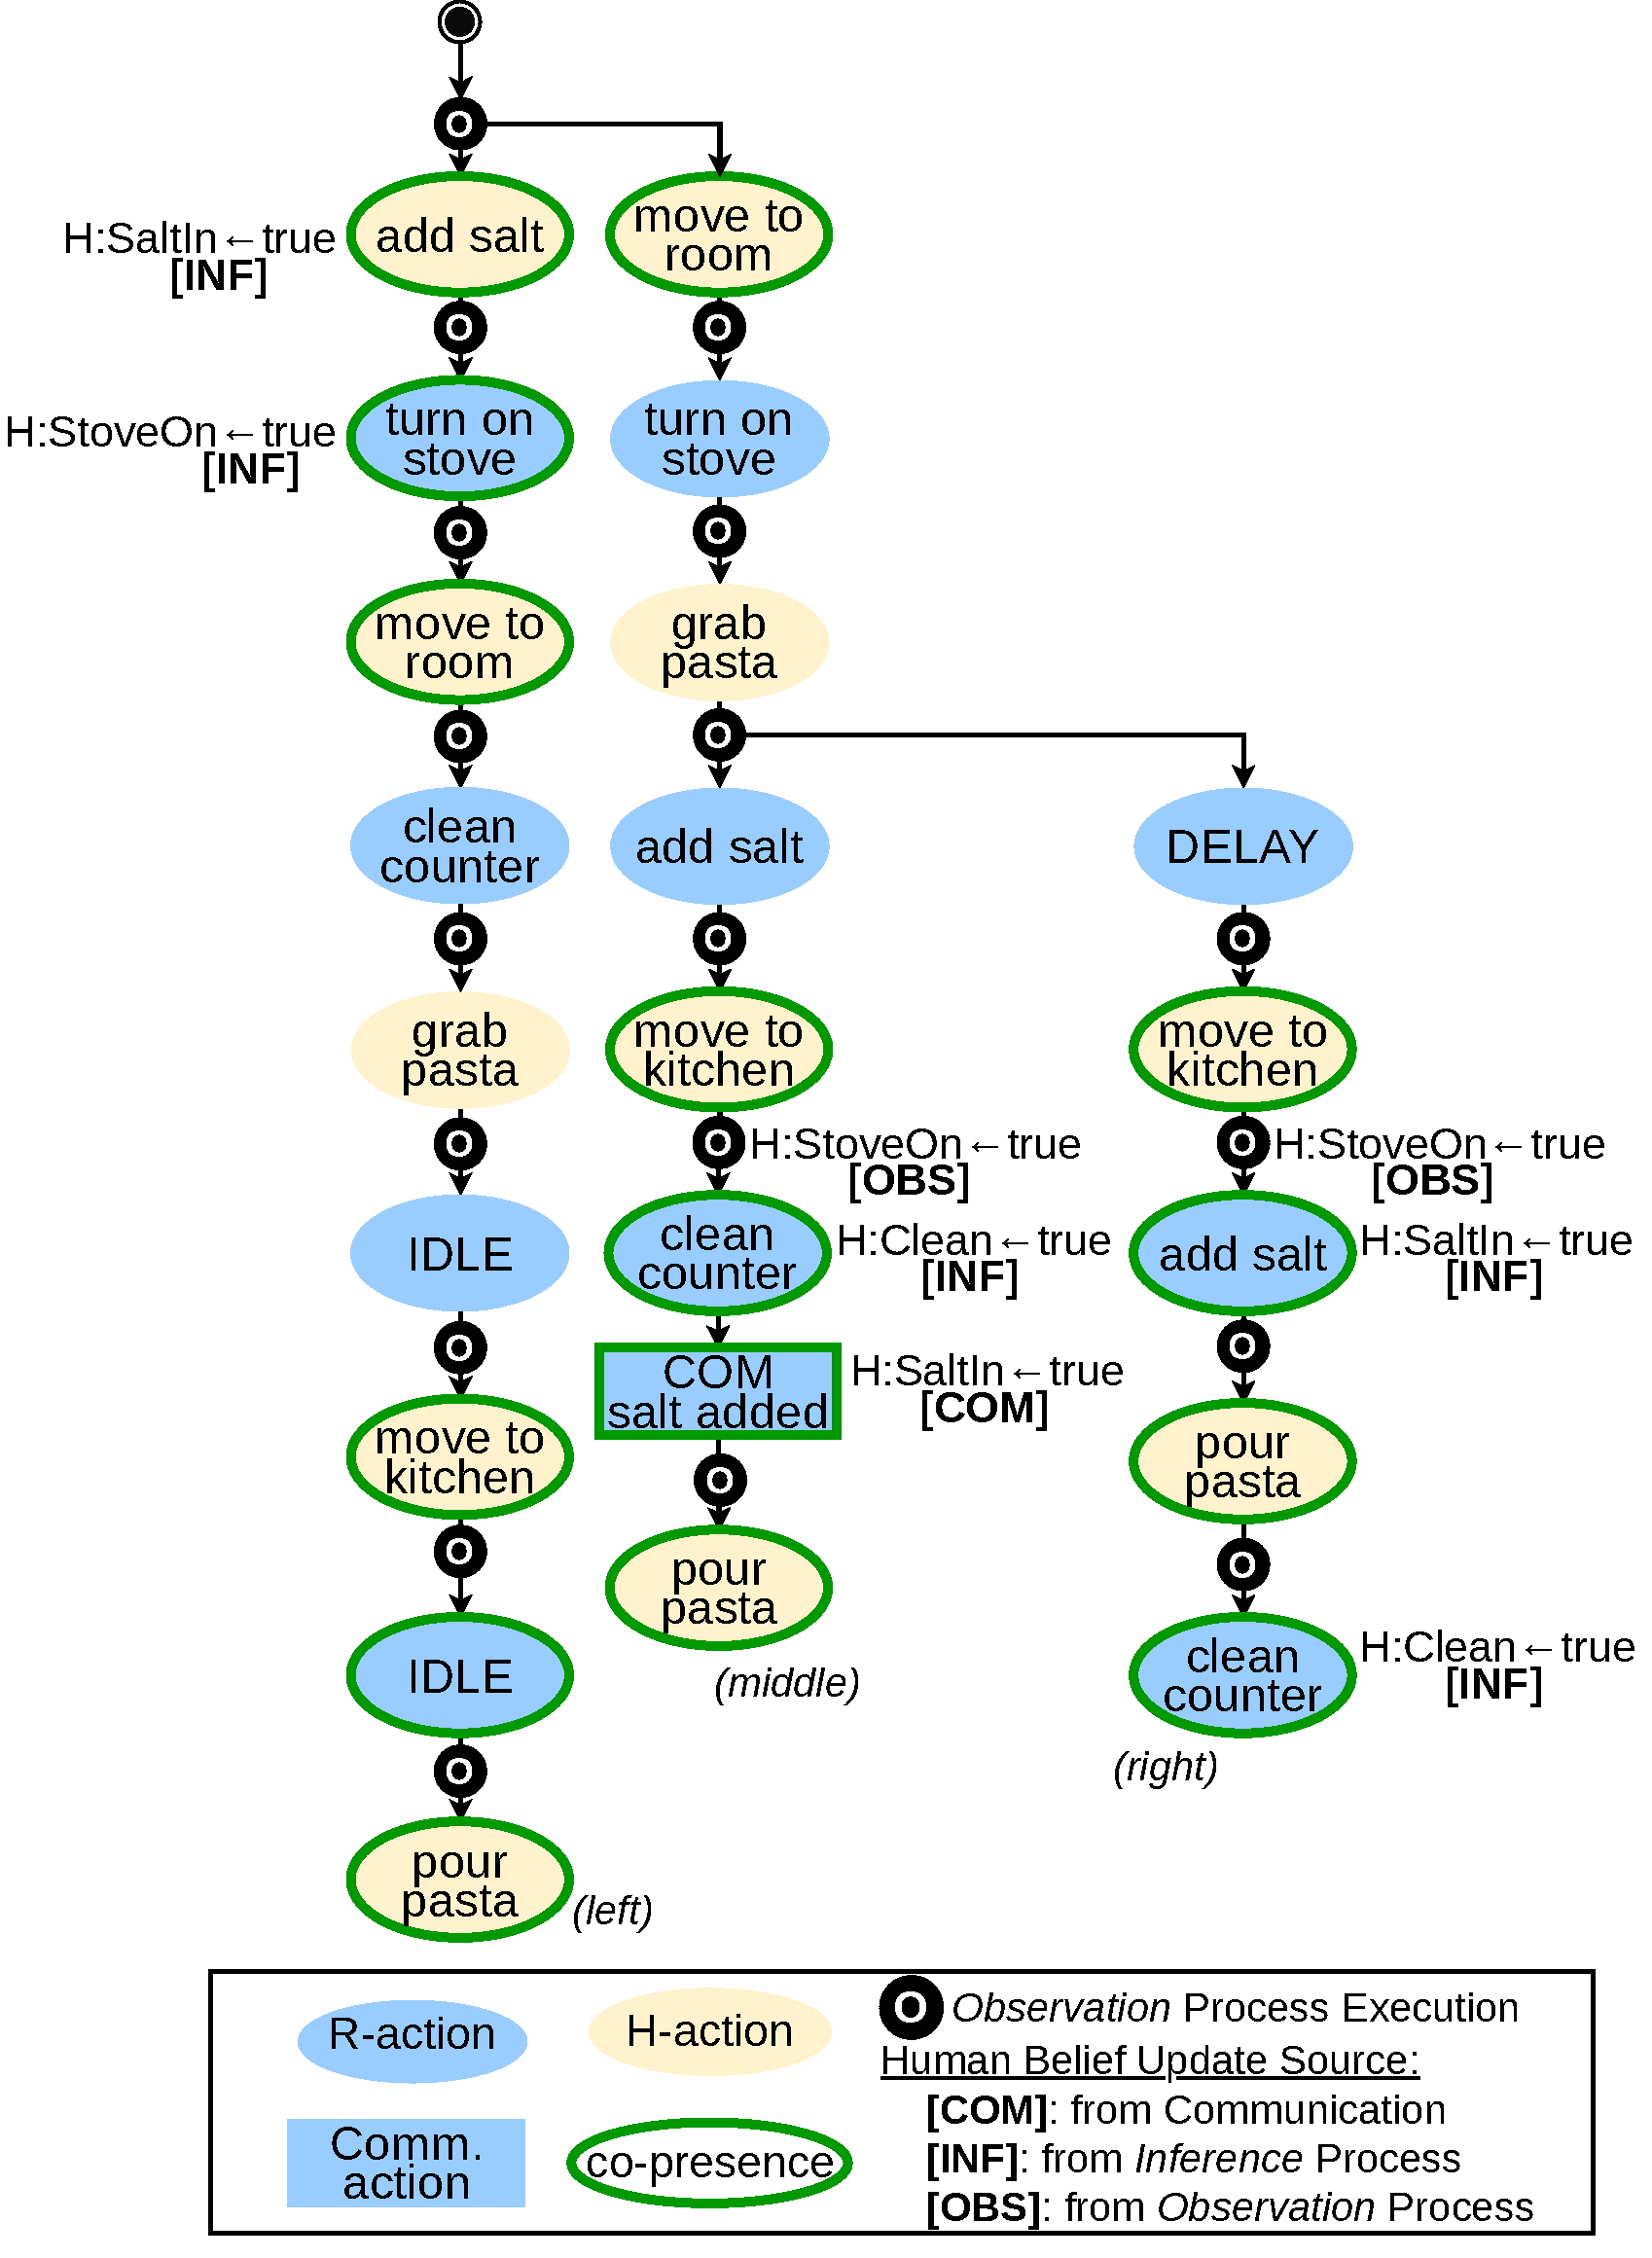
\includegraphics[width=0.65\linewidth]{images/Chapter3/plans.pdf}
    \caption{
    Plan obtained for the cooking scenario. 3 branches. Left: The human starts by adding salt. The only false belief is about \textit{``counterClean''} which is not relevant for the human agent, hence no comm is added. Middle: While the human is away the robot turns on the stove and adds salt, creating 2 false beliefs. 
    Once back, we estimate that the human agent
    will be able to assess the observable fact \textit{``stoveOn''} but not \textit{``saltIn''}. Since the human agent might add salt again due to this false belief, it is relevant and fixed with a communication action. Right: The relevant false belief about \textit{``saltIn''} is avoided by delaying the robot's action until the human is co-present.
    }
    \label{fig:cooking_plan}
\end{figure}

Considering the cooking domain, we discuss in detail the plans obtained with our approach to a problem corresponding to the description given in the introduction. 
I.e., there is no initial human false belief, agents both start in the kitchen, the pasta is in the adjacent room, the stove is off, and there is no salt in the water. The resulting plans are shown in Fig.~\ref{fig:cooking_plan} and their detailed presentation explains how the approach works in practice. 
Since human is uncontrollable and has different possible actions, the plan branches and the robot's actions are different in each case. 

In (\textit{left}) the human first adds salt and then the robot turns on the stove. In both cases, thanks to the inference process, we estimate that the human will be aware of both facts about the salt (\textit{acting}) and the stove (\textit{co-present}). Then while the human is away to fetch the pasta, the robot cleans the counter and since the human isn't co-present their beliefs aren't updated, containing now a false belief. Once back, since \textit{counterClean} is not \textit{observable} the observation process does nothing and the false belief remains. However, this false belief doesn't affect human actions (non-relevant), hence, there is no need to align human beliefs.

In (\textit{middle} and \textit{right}) the human first fetches the pasta by leaving the kitchen. Let's first focus on the (\textit{middle}) trace. The robot turns on the stove and adds salt while the human is away, creating two false beliefs. When returning to the kitchen, the observation process updates the human beliefs with the observable facts located in the kitchen. This fixes the false belief about \textit{stoveOn}. The robot then cleans the counter, observed by the human. 
However, without communication, the human's next action will be either ``add salt'' or ``ask the robot'', but considering the ground truth the human could directly pour the pasta. Hence, the false belief on \textit{saltIn} is relevant and has to be corrected. To do so a communication is inserted in the robot's plan and a ``delay'' branch is created (\textit{right}). 
In this delaying branch, the robot delays the add salt action until the human is co-present in order to make it observed (inference process) by the agent. 
In addition to this implicit communication, like in (\textit{middle}), the human assesses that the stove is on and hence can directly pour the pasta. 
\begin{table}[t]
    \centering
    \vspace{0.1cm}
    \caption
    {
    Success and communication ratio of different approaches. 
    }
    \label{tab:q_results}
    \begin{tabular}{@{}c|c c|| c| c@{}}
    % \begin{tabular}{c|c c|| c}
        \multirow{2}{*}{\textbf{Domain}} & \multicolumn{2}{c||}{\textbf{HATP/EHDA}} & \multicolumn{1}{c|}{\textbf{Only Comm}} & \multicolumn{1}{c}{\textbf{With Delay}}
        \\
        & \multicolumn{1}{c}{\textit{S}} & \multicolumn{1}{c||}{\textit{S I.Div.B.}} & \multicolumn{1}{c|}{\textit{Comm}} & \multicolumn{1}{c}{\textit{Comm}} 
        \\ \cline{1-5}
        \textit{Cooking}    &   18.6\%  &  6.9\%    & 69.5\% & 65.2\%\\
        \textit{Box}        &   25.0\%  & 14.3\%    & 79.7\% & 75.0\%\\
        \textit{Car}        &   12.5\%  & 0.0\%     & 68.8\% & 64.1\%\\
        \hline
        \textbf{Average}    &   18.7\%  & 7.1\%     & 72.6\% & 68.1\%\\
    \end{tabular}
\end{table}

\subsection{Experimental Results and Analysis}

In each domain, the actions and tasks remain the same. So here, a problem is defined by a starting agent ($R$ or $H$) and a pair of initial beliefs ($val^R_0, val^H_ 0$).
Initial ground truth ($val_0 \Leftrightarrow val^R_0$) is defined by setting each state variable to an initial value. But, 5 selected state variables can be set to 2 possible values instead of 1. Among these selected ones, 3 can diverge in human belief. This generates 256 pairs of initial beliefs where 12.5\% of them include initially aligned beliefs. Then, considering the starting agent, we obtain 512 problems for each domain. 
Each of the 1536 generated problems has been solved by HATP/EHDA, by \textit{our approach} using first \textit{only communication} and then using also \textit{delay}.
The obtained quantitative results appear in TABLE~\ref{tab:q_results}.
 
The overall success rate ($S$) and the one for initially diverging beliefs ($S I.Div.B.$) are shown for the HATP/EHDA solver. As expected, this solver always finds legal plans when dealing with initially aligned beliefs, but the low value of $S I.Div.B.$ reflects how poorly it handles belief divergences without specifically designed action models.
Our approach always finds legal plans so we omitted its success rates in the last two columns, and we can say that it solves a broader class of problems.

Furthermore, considering the initially diverging beliefs and the divergences created along the planning process, more than $87.5\%$ of all problems involve belief divergences. 
However, when using only verbal communication, only $72.6\%$ of the generated plans include communication actions.
This means that \textit{our approach} communicates only when necessary, and not systematically. 
The amount of communication is even reduced to $68.1\%$ when delaying actions. In the latter case, only delayed branches that do not imply the human to wait are kept. 

%%% SECTION %%%%%%%%%%%%%%%%%%%%%%%%%%%%%%%%%%%%%%%%%%%%%%%%%%%%
\section{Discussion and Limitations}

The underlying scheme allows just a single agent to execute a \textit{``real''} action at a time. 
However, a post-process can allow the execution of actions concurrently~\cite{CrosbyJR14}, however, note that the domain modeler has modeled $\mathcal{P}_{rh}$ as a sequential joint task. 
Parallelism is not considered in the current modeling and planning process, which limits the potential for concurrent executions. However, we are working on extending the framework to enable systematic planning with concurrent actions, aligning with~\cite{ShekharB20}.

We believe our modeling-level SA proposals could fit in any other planning approach framing multi-party systems having one controllable agent while can only hypothesize remaining agents' behaviors (e.g., human-centered AI).

Agents' SA models cannot simply refute a false belief, they can only assess new true facts to correct them.
E.g., assume the human \textit{wrongly} believes that the pasta is in \textsf{kitchen}. The SA does not help refute this when the agent is in \textsf{kitchen}
because appropriate knowledge reasoning w.r.t. \textit{NotAt(Pasta)} in \textsf{kitchen} is not taken into account.  
However, such issues do not affect the completeness and, if necessary, our approach \textit{tackles} such cases as relevant false beliefs.

We have planned a user study for the future to conform our framework with reality and validate the approach.

We discussed earlier that DEL knowledge representation is more expressive and flexible, and can handle uncertainty. However, it requires an augmented action schema to accurately maintain each agent's beliefs.
Think of a specification for \textit{``move''} action manually listing all the environmental facts to be observed by an agent for managing their beliefs. In our case, it is implicitly maintained within a state.

We can consider running a set of rules (e.g., \textit{graph-based ontology}) to bring new interesting facts in the state based on a set of known facts. We believe that this aspect opens up new possibilities in the future to integrate human-aware collaborative planning and ontology.

%%% SECTION %%%%%%%%%%%%%%%%%%%%%%%%%%%%%%%%%%%%%%%%%%%%%%%%%%%%
\section{Epistemic Extension}

The planning process proposed in this contribution is part of the epistemic planning field. However, the uncertainties are limited and focused on the human decisions, in a simplistic manner compared to ``classical'' epistemic planner. Indeed, state-of-the-art epistemic planners consider epistemic states rather than ``simple'' beliefs and thus are able to keep track of several possible worlds. More precisely, [cite bolander] this work using the DEL approach are able to keep track and reason on several possible worlds for each agent, and can even manage distinguishable worlds from others. Hence, the planner is able to anticipate that an agent can believe in three different possible worlds and tell that at execution time the agent will be able to distinguish if they are in world 1 or not, but they will not be able to tell distinguish between world 2 and 3 (based on observable facts).
Such approaches currently heavily rely on conditional action effects and scripting. That is, when an agent enters a room with an action \textit{move}, the \textit{move} conditional effects will update accordingly the agent's possible worlds (the agent sees a box, notice that someone isn't in the room anymore, and so on...). These situation assessment rules must be encoded into the action model used, and more precisely, in the action's effect which isn't convenient and is domain specific.
Our contribution proposes generalized situation assessment rules to maintain the beliefs but at the price to have simplified epistemic states.

In some preliminary work we explored an extension of our approach to handle such classical epistemic representation. 

* Describe first findings and models * 

* Some results ? *

* Discuss limitations: the current design is computationally very expensive and doesn't scale. Work on this aspect are needed and in progress to continue investigating this extension * 


%%% SECTION %%%%%%%%%%%%%%%%%%%%%%%%%%%%%%%%%%%%%%%%%%%%%%%%%%%%
\section{Conclusion}

We propose an extension to a Human-Aware Task Planner called HATP/EHDA. 
The planner plans and implicitly coordinates the robot's actions with all estimated possible human (uncontrollable) behaviors that are then emulated to generate a new state.
Our extension and contribution are, first, to integrate a \textit{Situation Assessment} based reasoning system in the planner. This allows for maintaining distinct agents' beliefs based on what they can/should observe.
Compared to existing epistemic planners, this simplifies the action descriptions by focusing on their effects on the world, and not how they influence each agent's beliefs.
In addition, we propose to detect false human beliefs and tackle only the necessary ones in a principled way. First, we propose minimal and proactive explicit communication. Second, when pertinent, 
we propose an implicit communication by postponing the non-observed robot action until the human is co-present to observe it.  

The relevance of false belief, when to optimally communicate and parallelization are interesting future works, and we aim at conducting a user study to validate the benefits of the proactive robot behavior that our approach permits. 